\section{واحد شمارشگر (\lr{Counter})}
در این بخش، یک واحد شمارشگر ۳۲ بیتی را با رویکرد درختی طراحی کردیم که قادر است تعداد صفرهای ابتدایی (\lr{CLZ})، صفرهای انتهایی (\lr{CTZ})، یک‌های ابتدایی (\lr{CLO}) و یک‌های انتهایی (\lr{CTO}) را محاسبه کند.

مطابق صورت تمرین، ورودی‌ها و خروجی‌های این واحد به این صورت هستند:
\begin{itemize}
    \item \textbf{ورودی‌ها:}
          \begin{enumerate}
              \item \textbf{\lr{\code{Data}}}: داده ورودی برای واحد شمارشگر (32 بیت)
              \item \textbf{\lr{\code{Count\_Op}}}: انتخاب نوع عملیات شمارش (2 بیت)
          \end{enumerate}

    \item \textbf{خروجی:}
          \begin{enumerate}
              \item \textbf{\lr{\code{Count}}}: تعداد بیت‌های شمارش شده توسط واحد شمارشگر (6 بیت - عددی بین 0 تا 32)
          \end{enumerate}
\end{itemize}

عملیات متناظر با هر کد کنترلی در جدول زیر آمده است:

\begin{table}[H]
    \centering
    \caption{دستورات شمارش بیت‌ها}
    \vspace{0.2cm}
    \begin{tabular}{|c|c|c|}
        \hline
        \textbf{کد کنترلی} & \textbf{نام دستور} & \textbf{شرح عملیات}                    \\
        \hline
        $00$               & \lr{CTZ}           & شمارش تعداد بیت‌های 0 در سمت کم‌ارزش عدد \\
        \hline
        $01$               & \lr{CTO}           & شمارش تعداد بیت‌های 1 در سمت کم‌ارزش عدد \\
        \hline
        $10$               & \lr{CLZ}           & شمارش تعداد بیت‌های 0 در سمت پرارزش عدد \\
        \hline
        $11$               & \lr{CLO}           & شمارش تعداد بیت‌های 1 در سمت پرارزش عدد \\
        \hline
    \end{tabular}
\end{table}

\subsection{طراحی ماژول پایه (\code{CTZ\_8bit})}
پیش از ساخت مدار ۳۲ بیتی، ابتدا یک شمارشگر صفر انتهایی ۸ بیتی (\lr{CTZ}) ساختیم. این مدار با پیاده‌سازی یک درخت جستجوی دودویی (\lr{Binary Search Tree}) به کمک گیت‌های \code{OR} طراحی شده است. در هر مرحله، بازه‌ها نصف شده و در صورتی که نیمه کم‌ارزش کاملاً صفر باشد، به سراغ نیمه پرارزش می‌رود. خروجی گیت‌های \code{OR}، خطوط انتخابِ (\lr{Select}) مالتی‌پلکسرها را کنترل می‌کنند. همچنین خروجی \lr{\code{all\_z}} نیز نشان‌دهنده‌ی صفر بودن کل ۸ بیت است.
از آنجا که این بخش تنها از گیت‌های موازی \code{OR} با عمق ۳ و مالتی‌پلکسر تشکیل شده، تاخیر آن مقدار ثابتی است (\lr{$O(1)$}).

\begin{figure}[H]
    \centering
    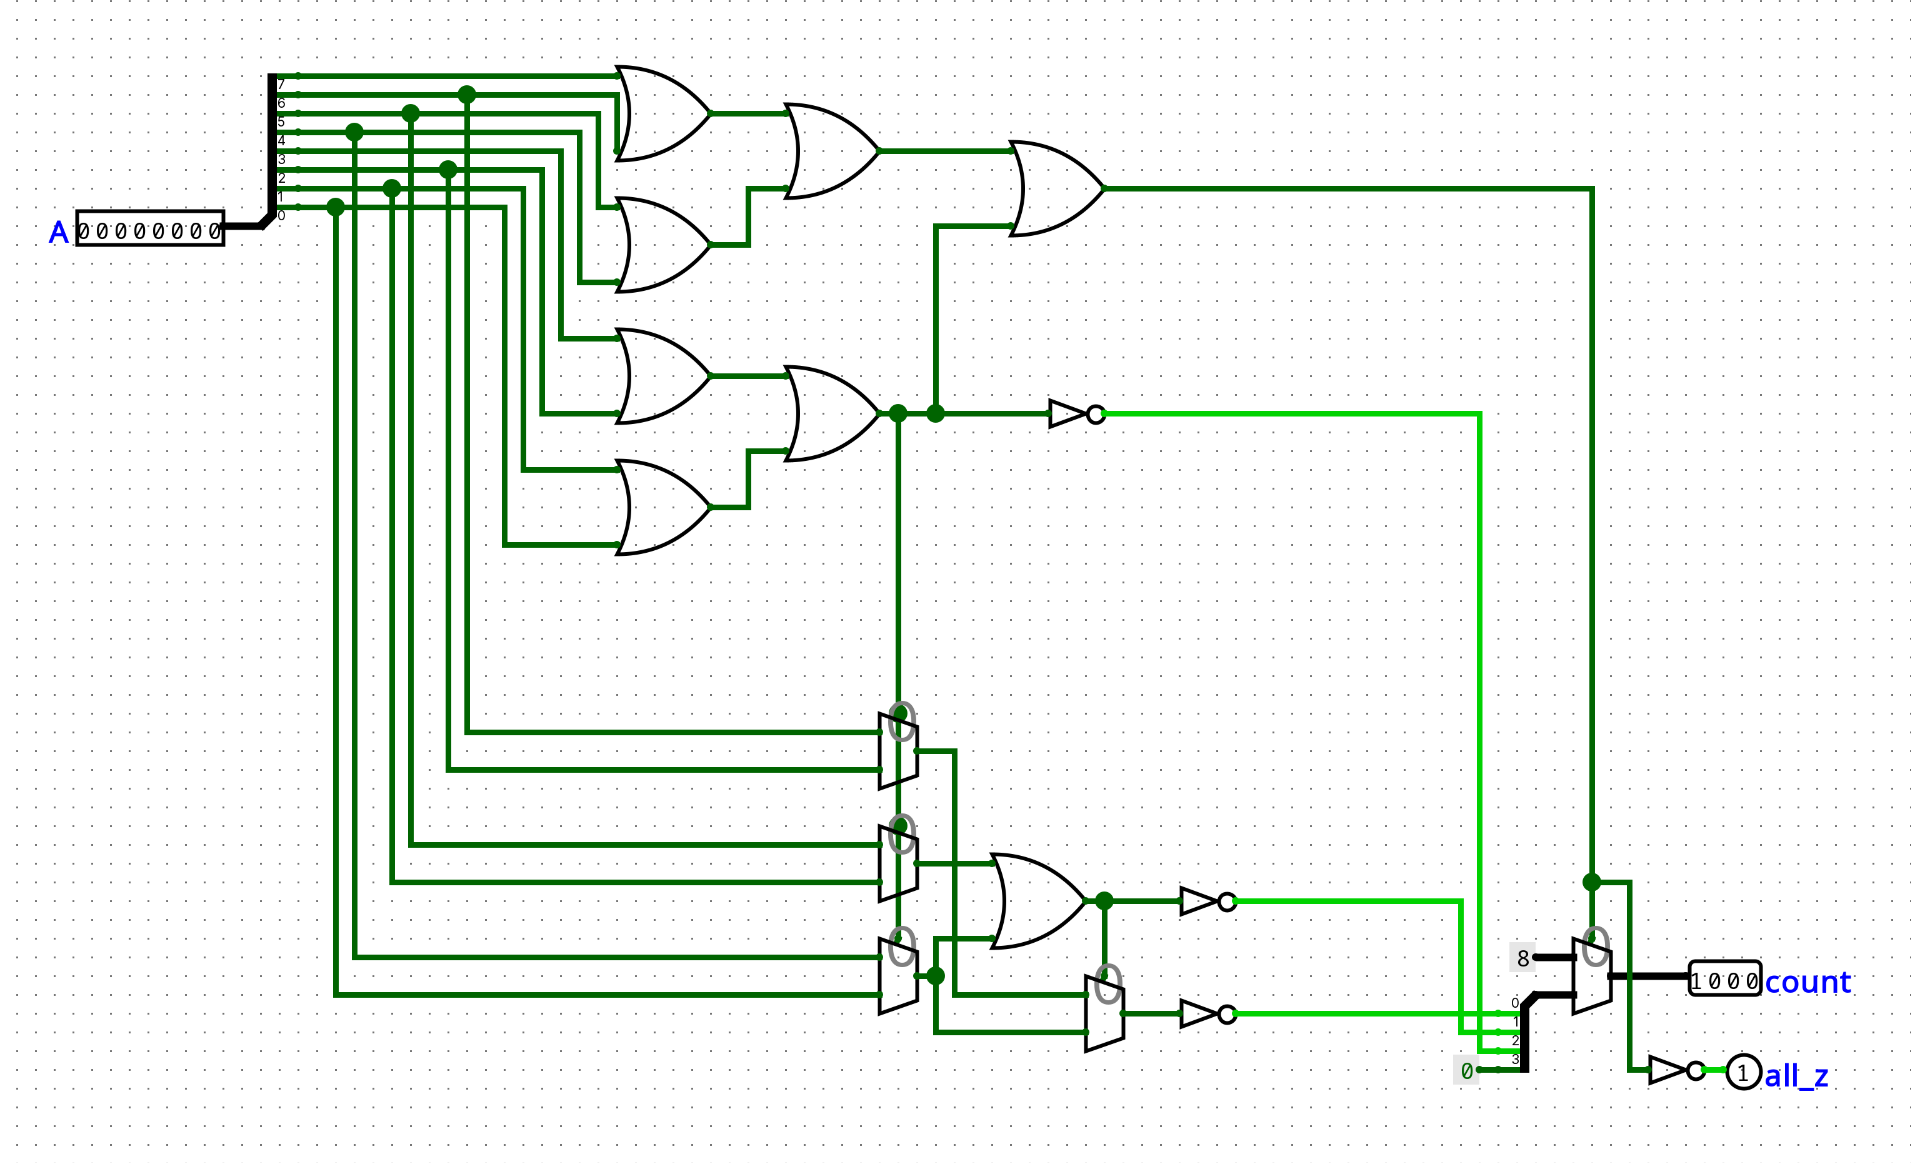
\includegraphics[width=1.0\textwidth]{assets/CTZ_8bit.png}
    \caption{پیمانه‌ی \code{CTZ\_8bit}}
\end{figure}

\subsection{توسعه‌ی درختی (\code{CTZ\_16bit} و \code{CTZ\_32bit})}
برای ساخت مدار ۱۶ بیتی از ترکیب دو مدار ۸ بیتی (\lr{Lo} و \lr{Hi}) استفاده کردیم. در اینجا از ترکیب سیگنال‌ها با استفاده از \lr{Splitter} استفاده کردیم.
اگر بخش \lr{Lo} کاملاً صفر باشد (سیگنال \lr{\code{all\_z}} برابر یک)، خروجی بخش \lr{Hi} انتخاب می‌شود و در غیر این صورت خروجی \lr{Lo}. در صورت انتخاب بخش \lr{Hi}، عدد ۱ به جایگاه بیت چهارم (با ارزش ۸) متصل می‌شود که معادل جمع با ۸ است، بدون آنکه تاخیر محاسبه‌ی جمع به مدار تحمیل شود. توسعه‌ی مدار ۳۲ بیتی نیز دقیقاً به همین شیوه با استفاده از دو بلوک ۱۶ بیتی انجام می‌شود.

\begin{figure}[H]
    \centering
    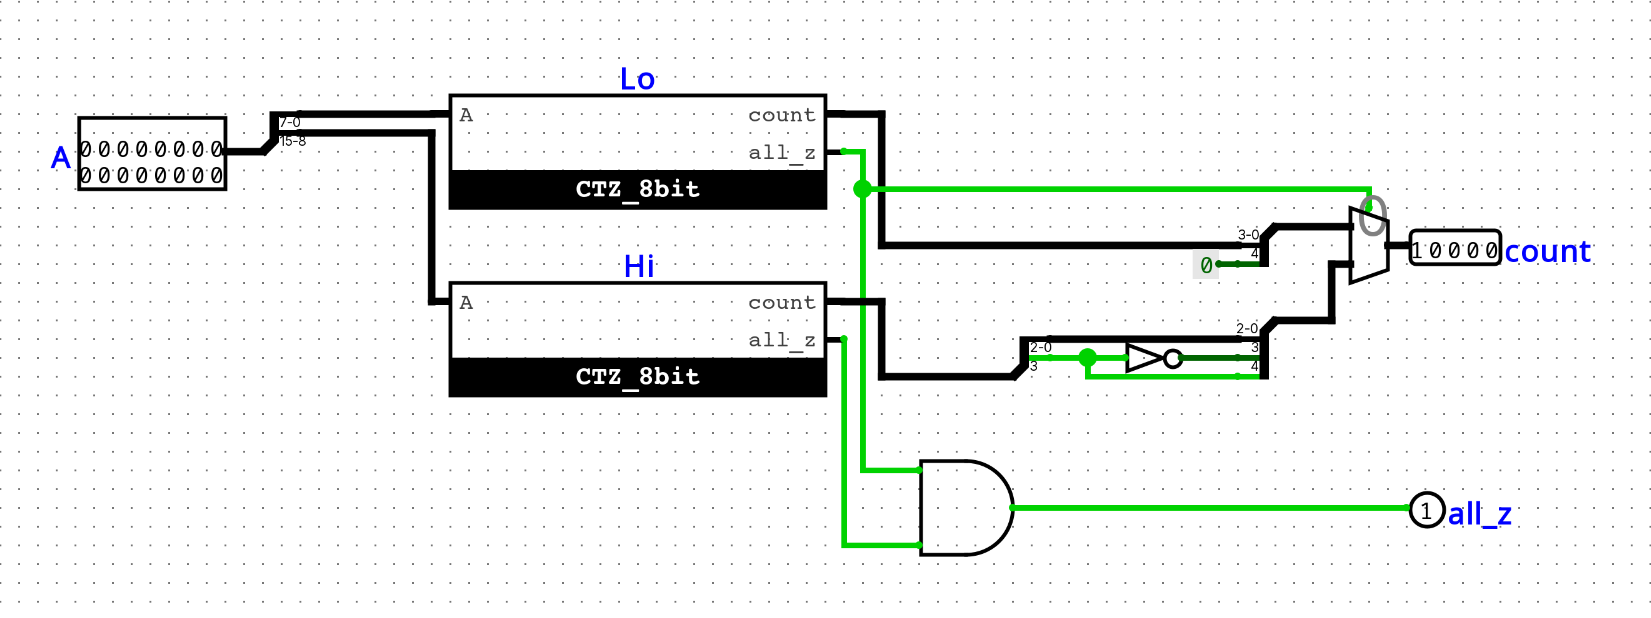
\includegraphics[width=0.8\textwidth]{assets/CTZ_16bit.png}
    \caption{توسعه‌ی پیمانه‌ی \code{CTZ\_16bit} بدون استفاده از جمع‌کننده}
\end{figure}

\begin{figure}[H]
    \centering
    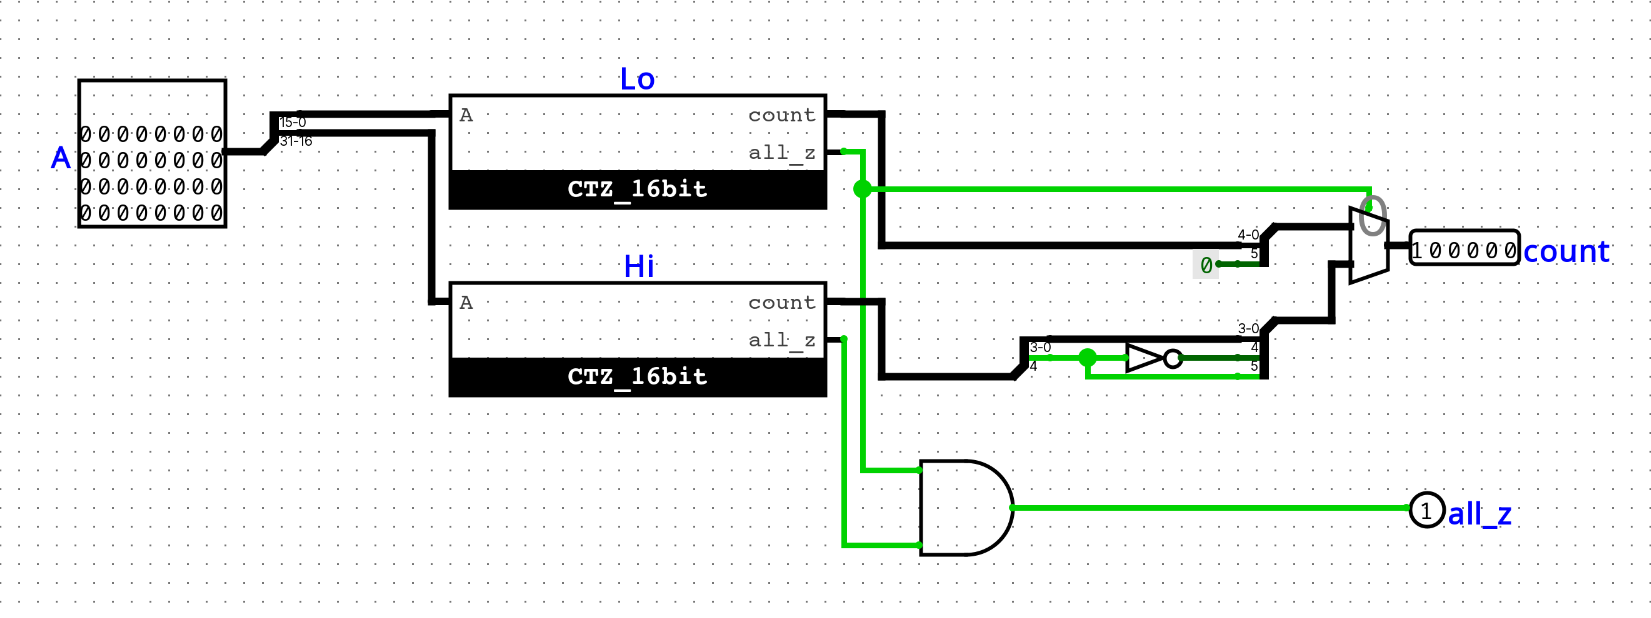
\includegraphics[width=0.8\textwidth]{assets/CTZ_32bit.png}
    \caption{پیمانه‌ی \code{CTZ\_32bit}}
\end{figure}

\subsection{پیش‌پردازش ورودی‌ها (\code{correction})}
برای پشتیبانی از عملیات \lr{CLZ} ،\lr{CLO} و \lr{CTO} بدون نیاز به افزودن سخت‌افزار تکراری، یک واحد اصلاح (\lr{Correction}) پیش از ورود داده به هسته‌ی \lr{CTZ} قرار دادیم.
اگر عملیات شمارش از سمت پرارزش (\lr{Leading}) باشد، به کمک ابزار \lr{Splitter} ترتیب بیت‌ها را معکوس می‌کنیم. اگر عملیات شمارش یک‌ها (\lr{Ones}) باشد، کل بیت‌ها توسط گیت‌های موازی \code{NOT} نقیض می‌شوند. این عملیات توسط مالتی‌پلکسرها و با توجه به پایه‌های \lr{\code{Count\_Op}} کنترل می‌گردد. از آنجایی که معکوس کردن تنها تغییر سیم‌کشی است و گیت‌های \code{NOT} موازی هستند، تاخیر این بخش نیز \lr{$O(1)$} است.

\begin{figure}[H]
    \centering
    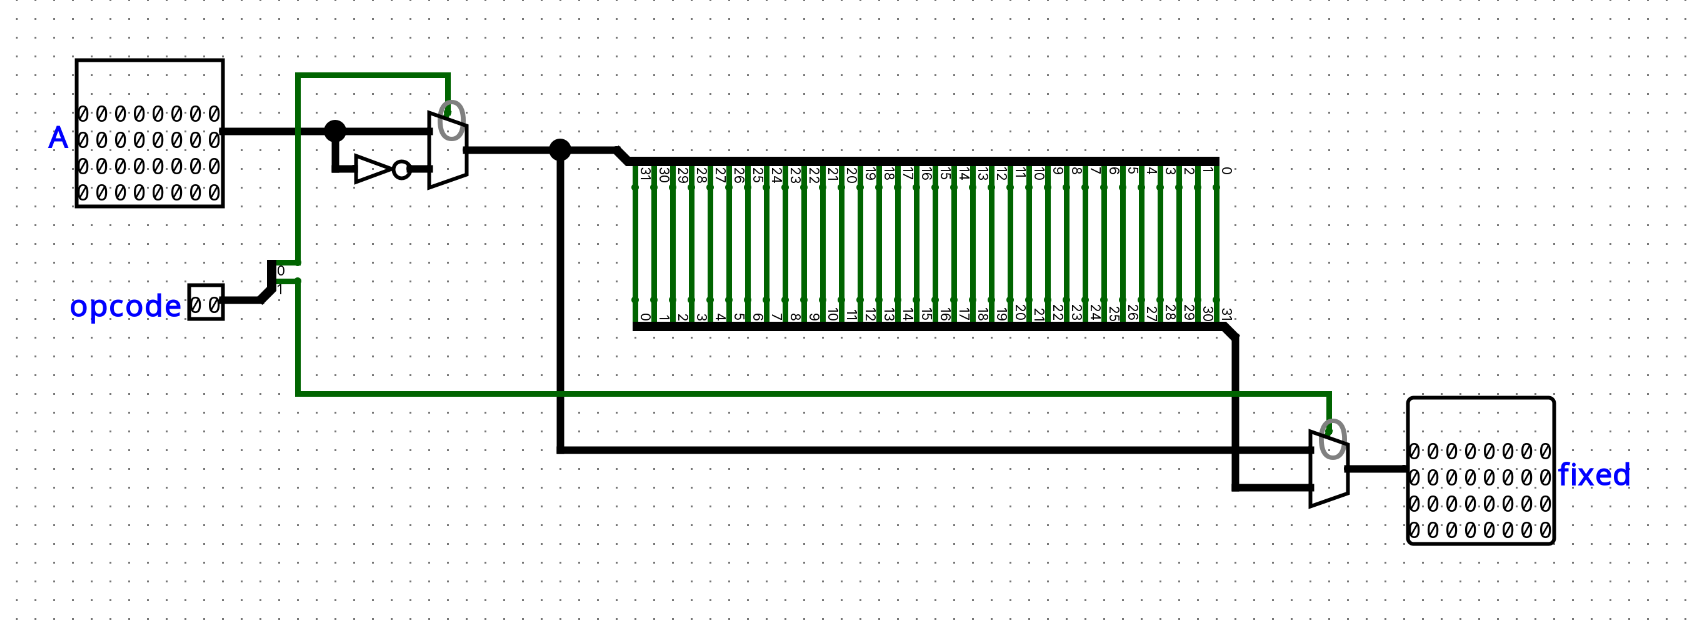
\includegraphics[width=1.0\textwidth]{assets/correction.png}
    \caption{واحد پیش‌پردازش و اصلاح داده‌ها (\code{correction})}
\end{figure}

در نهایت، با اتصال واحد تصحیح به هسته‌ی ۳۲ بیتی، مدار اصلی کامل می‌شود:

\begin{figure}[H]
    \centering
    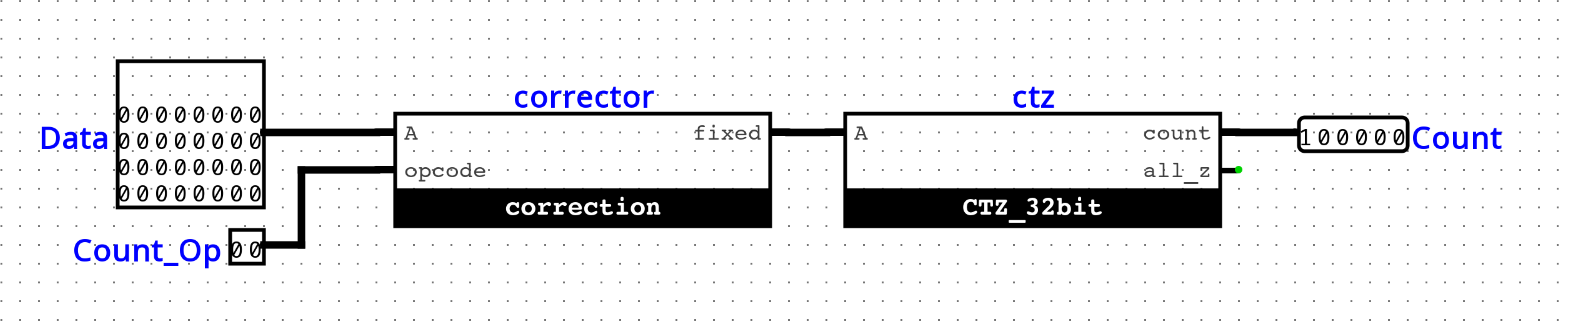
\includegraphics[width=0.8\textwidth]{assets/main.png}
    \caption{واحد کامل شمارشگر ۳۲ بیتی}
\end{figure}

\textbf{تحلیل تاخیر مدار شمارشگر:}
\begin{align*}
    \text{\lr{Delay}}_{\text{\lr{Counter}}} = \text{\lr{Delay}}_{\text{\lr{Correction}}} + \text{\lr{Delay}}_{\text{\lr{CTZ\_8bit}}} + 2 \times \text{\lr{Delay}}_{\text{\lr{MUX}}}
\end{align*}
از آنجایی که توسعه‌ی عرض داده از ۸ بیت به ۳۲ بیت با اضافه شدن لگاریتمی لایه‌های \lr{MUX} صورت گرفته است، تاخیر کلی سیستم از مرتبه‌ی \lr{$O(\log n)$} خواهد بود.

\subsection{اجرای آزمون}

\begin{figure}[H]
    \centering
    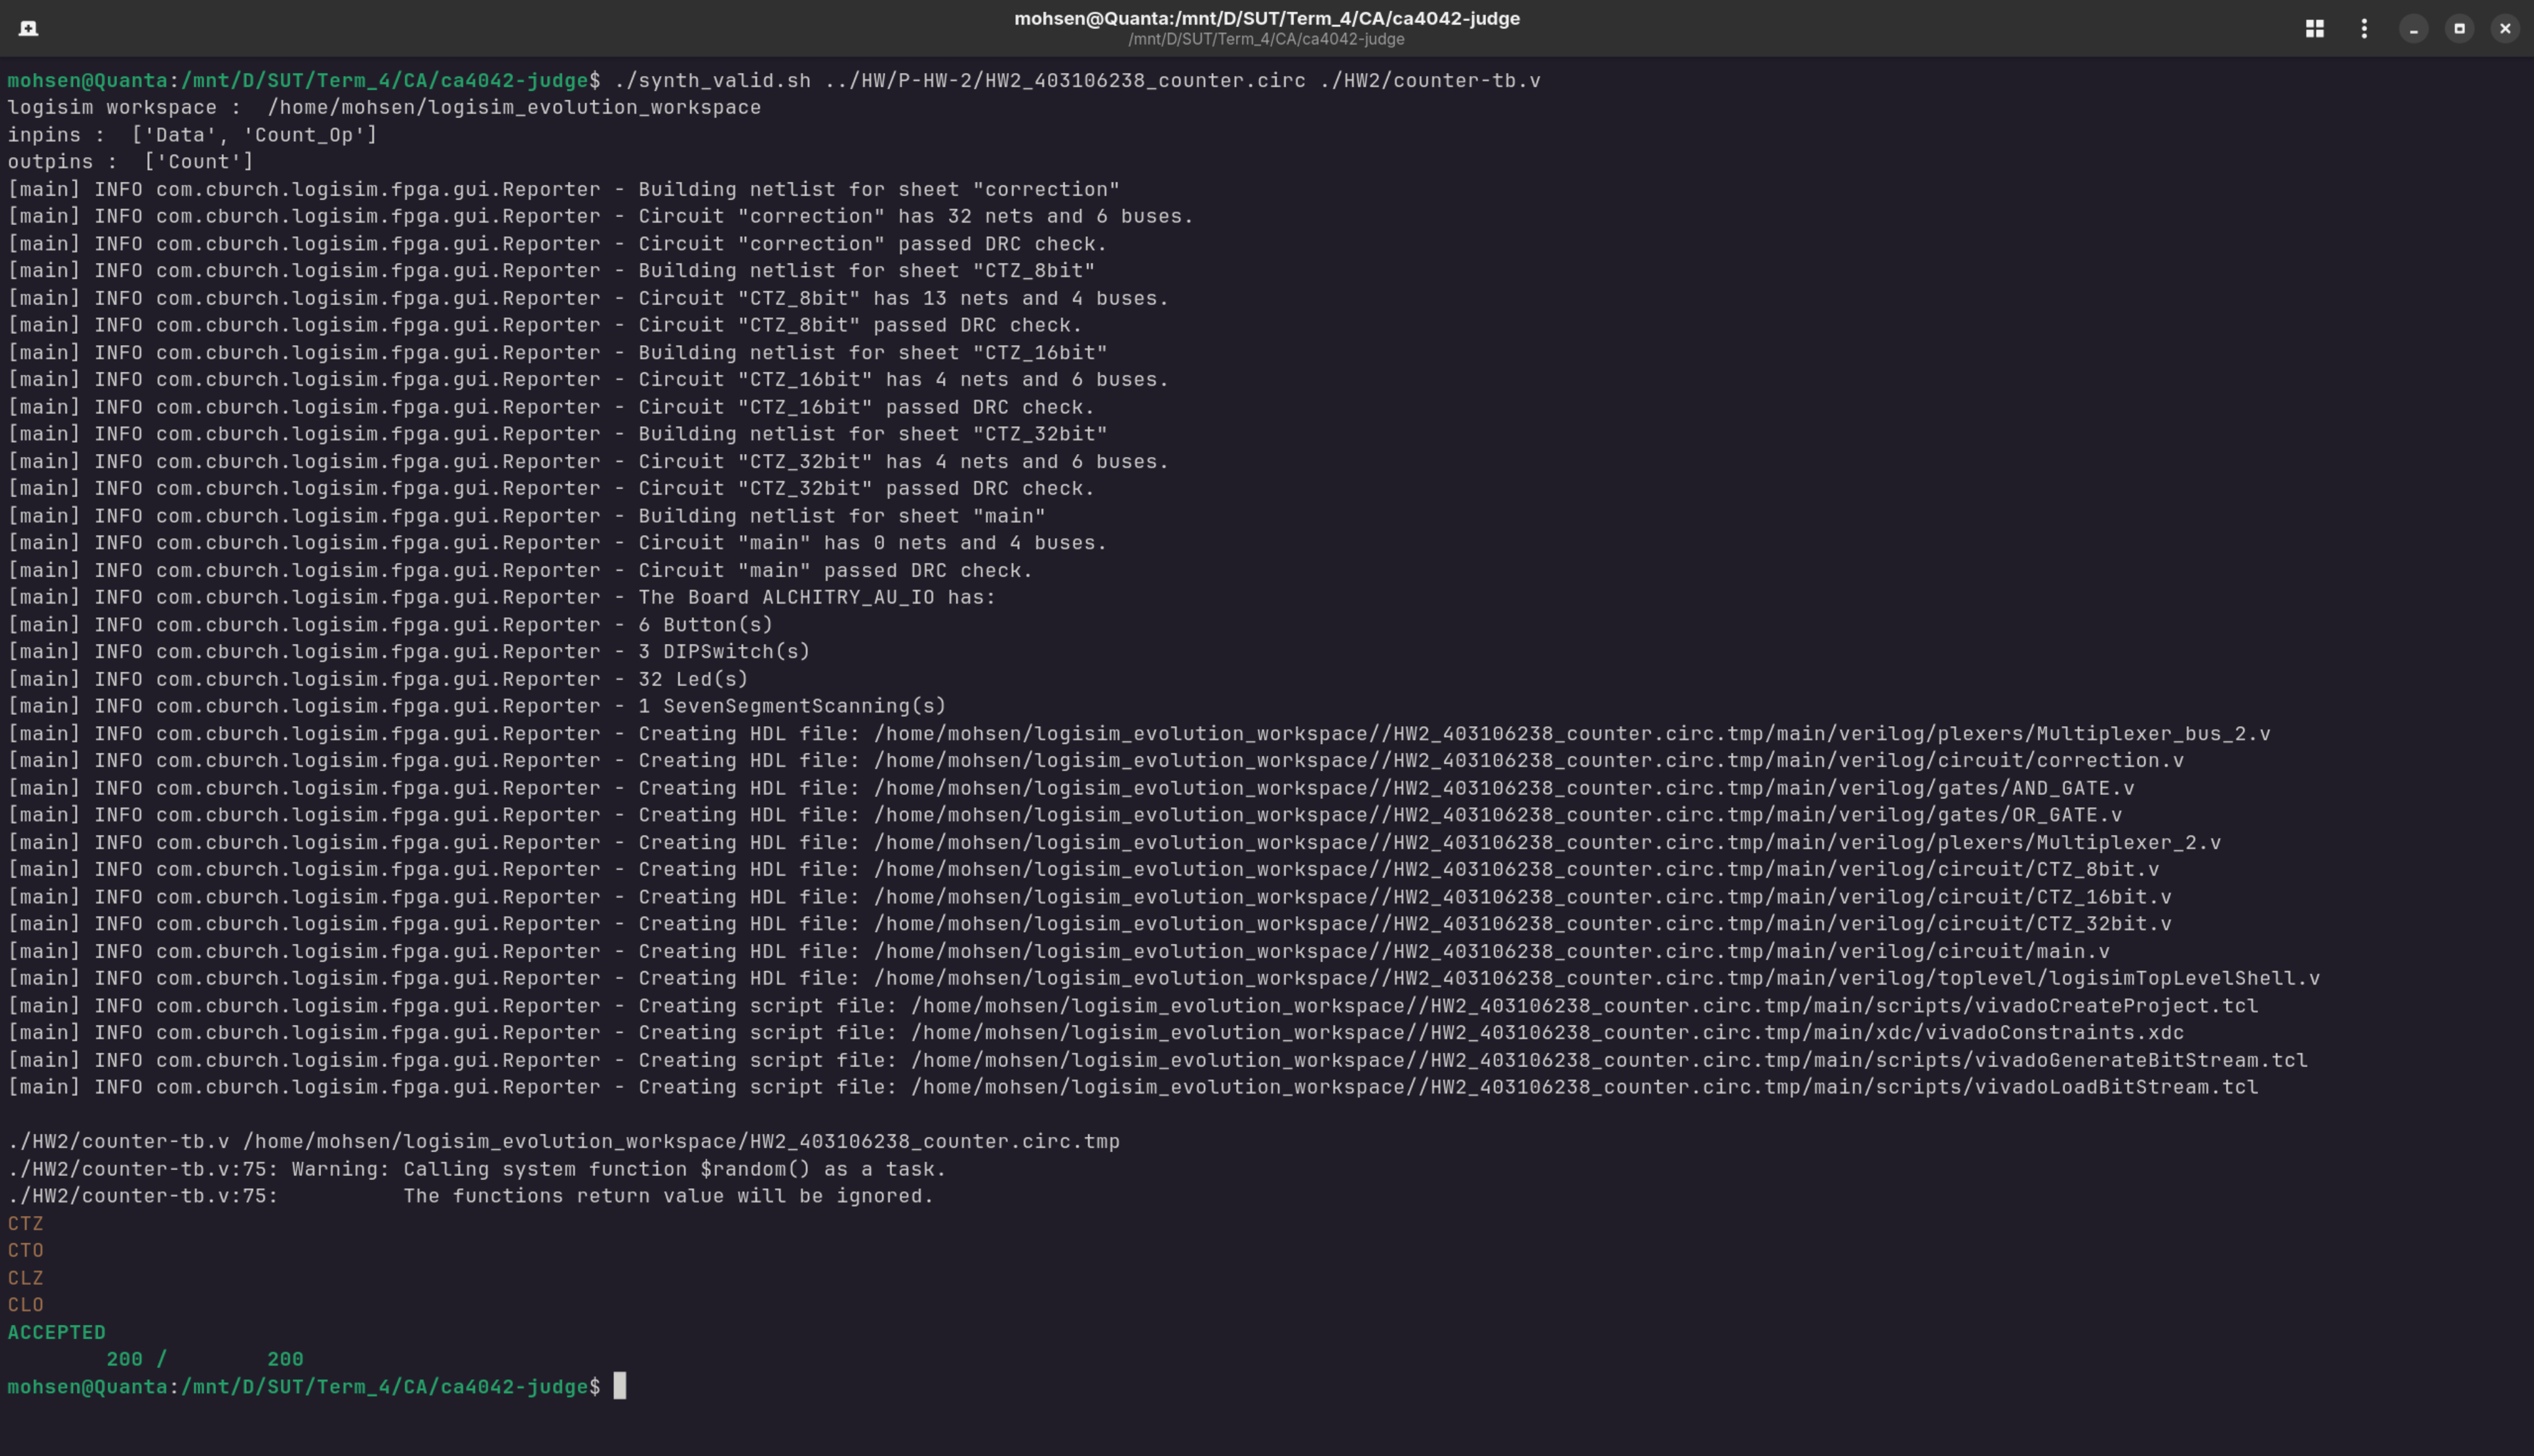
\includegraphics[width=1.0\textwidth]{assets/counter_test.png}
    \caption{تست مدار طراحی شده}
\end{figure}

\pagebreak

\section{واحد شیفت‌دهنده (\lr{Barrel Shifter})}
در این بخش، یک شیفت‌دهنده‌ی ۳۲ بیتی با ساختار لایه‌ای (\lr{Layered}) طراحی کردیم که قادر است عملیات شیفت منطقی به چپ، شیفت منطقی به راست و شیفت حسابی به راست را انجام دهد.

مطابق صورت تمرین، ورودی‌ها و خروجی‌های این واحد به این صورت هستند:
\begin{itemize}
    \item \textbf{ورودی‌ها:}
          \begin{enumerate}
              \item \textbf{\lr{\code{Data}}}: داده ورودی برای واحد شیفت‌دهنده (32 بیت)
              \item \textbf{\lr{\code{Shift\_Amt}}}: مقدار شیفت (5 بیت)
              \item \textbf{\lr{\code{Shift\_Op}}}: سیگنال کنترلی نوع شیفت (2 بیت)
          \end{enumerate}

    \item \textbf{خروجی:}
          \begin{enumerate}
              \item \textbf{\lr{\code{Result}}}: خروجی شیفت داده شده (32 بیت)
          \end{enumerate}
\end{itemize}

عملیات متناظر با هر کد کنترلی در جدول زیر آمده است:

\begin{table}[H]
    \centering
    \caption{دستورات شیفت‌دهنده}
    \vspace{0.2cm}
    \begin{tabular}{|c|c|c|}
        \hline
        \textbf{کد کنترلی} & \textbf{نام دستور} & \textbf{شرح عملیات}                  \\
        \hline
        $00$               & \lr{SLL}           & شیفت منطقی به چپ (پر کردن با صفر)    \\
        \hline
        $01$               & \lr{SRL}           & شیفت منطقی به راست (پر کردن با صفر)  \\
        \hline
        $10$               & \lr{SRA}           & شیفت حسابی به راست (تکرار بیت علامت) \\
        \hline
    \end{tabular}
\end{table}

\subsection{منطق طراحی و مسیر داده}
برای کاهش سخت‌افزار و جلوگیری از طراحی دو شبکه‌ی مجزا برای شیفت به چپ و راست، از تکنیک معکوس‌سازی بیت‌ها (\lr{Bit-Reversal}) استفاده شد. هسته‌ی اصلی مدار منحصراً کار شیفت به راست را انجام می‌دهد.
هنگامی که دستور شیفت منطقی به چپ (\lr{SLL}) دریافت شود، مقدار هر دو بیت کنترلیِ \lr{\code{Shift\_Op}} صفر است. با استفاده از یک گیت \code{NOR} متصل به این دو بیت، سیگنال معکوس‌سازی فعال شده و آرایش بیت‌های ورودی معکوس می‌شود. خروجی شیفت‌یافته نیز در انتهای مدار مجدداً معکوس می‌گردد تا شیفت به چپ شبیه‌سازی شود.

برای تولید بیت‌های جایگزین (پر کردن فضای خالی)، از یک مالتی‌پلکسر کنترل‌شده توسط \lr{\code{Shift\_Op[1]}} استفاده کردیم. در شیفت حسابی (\lr{SRA})، بیت جایگزین برابر با \lr{\code{Data[31]}} (بیت علامت) خواهد بود و در سایر حالات، مقدار ثابت صفر به لایه‌های شیفت‌دهنده تزریق می‌شود.

هسته‌ی شیفت‌دهنده از ۵ لایه (\lr{Stage}) تشکیل شده است که هر لایه شامل ۳۲ مالتی‌پلکسر است. پایه‌ی انتخاب (\lr{Select}) مالتی‌پلکسرهای لایه‌ی $i$ام به بیت $i$ام از سیگنال \lr{\code{Shift\_Amt}} متصل است. اگر این بیت یک باشد، داده‌ها به اندازه $2^i$ واحد شیفت پیدا می‌کنند و در غیر این صورت، بدون تغییر به لایه بعد منتقل می‌شوند.

\begin{figure}[H]
    \centering
    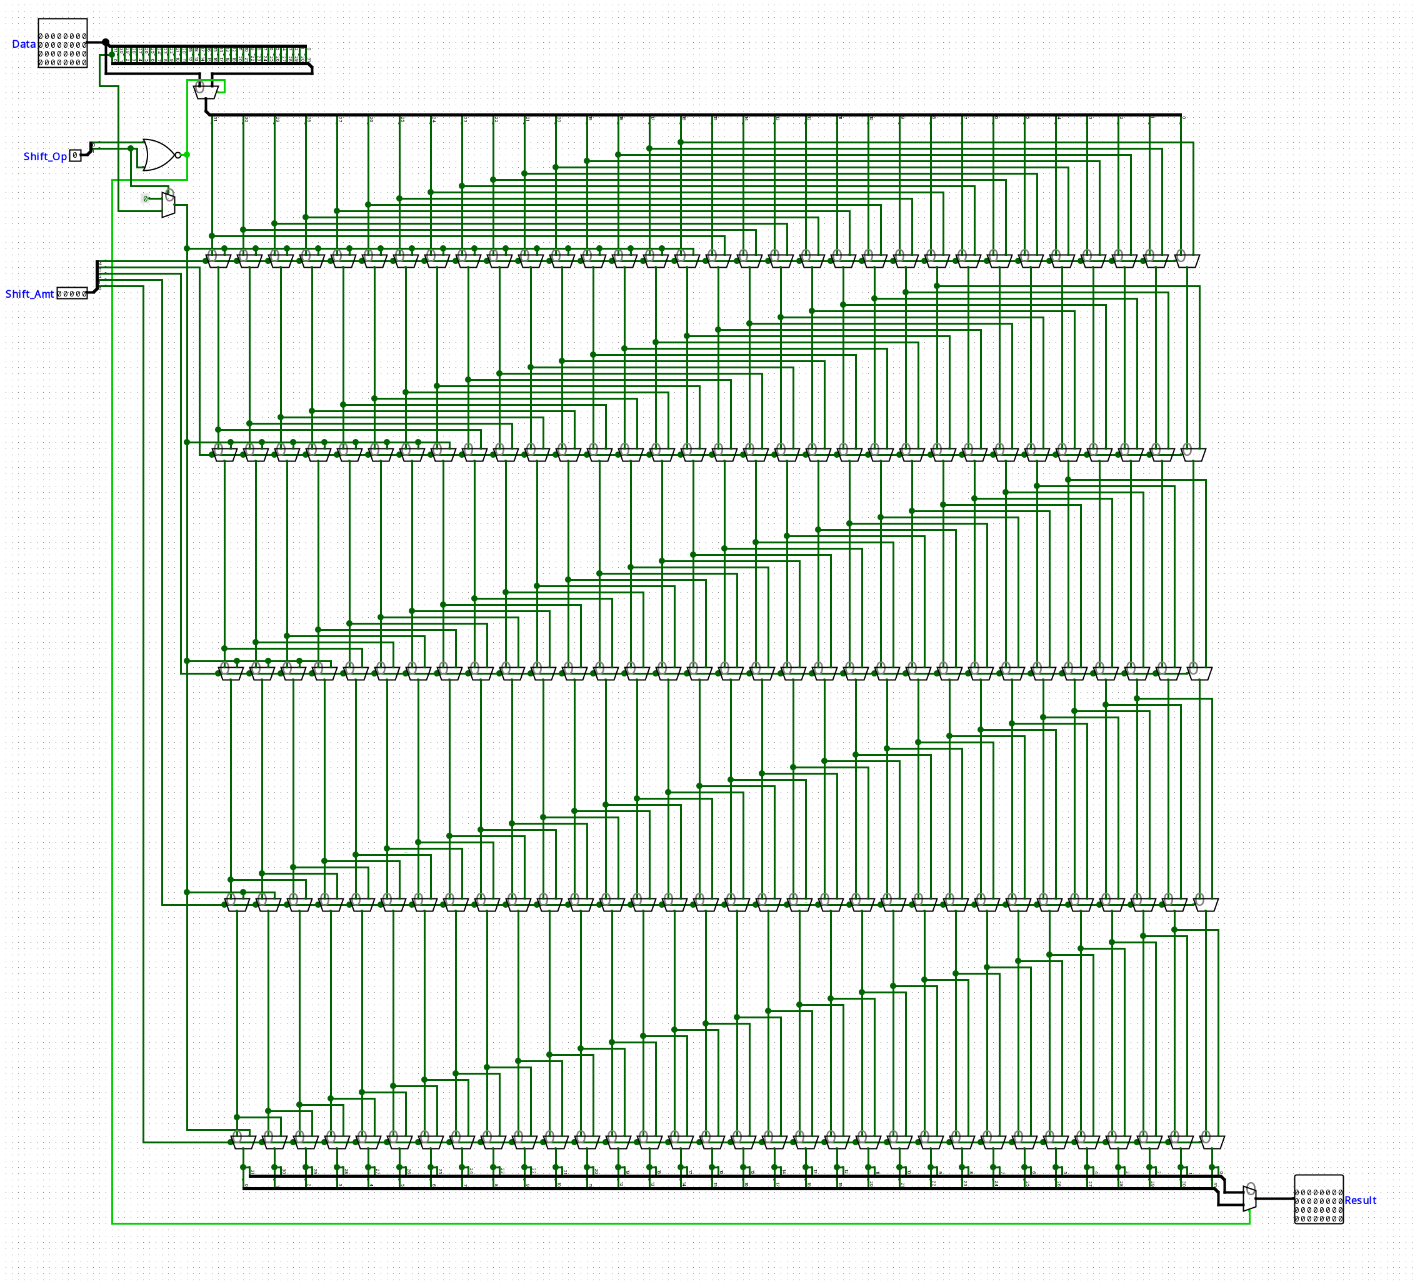
\includegraphics[width=1.0\textwidth]{assets/shifter.png}
    \caption{مدار شیفت‌دهنده‌ی لایه‌ای ۳۲ بیتی (\lr{Barrel Shifter})}
\end{figure}

\textbf{تحلیل تاخیر مدار شیفت‌دهنده:}
\begin{align*}
    \text{\lr{Delay}}_{\text{\lr{Shifter}}} = \text{\lr{Delay}}_{\text{\lr{Pre-Reversal}}} + \text{\lr{Delay}}_{\text{\lr{Layers}}} + \text{\lr{Delay}}_{\text{\lr{Post-Reversal}}}
\end{align*}
پیش‌پردازش و پس‌پردازش معکوس‌سازی هر کدام تنها نیازمند ۱ تاخیر مالتی‌پلکسر هستند. شبکه‌ی اصلی نیز داده را از ۵ لایه متوالی \lr{MUX} عبور می‌دهد (برابر با $\log_2(32)$). در نتیجه، تاخیر مدار شیفت‌دهنده از مرتبه \lr{$O(\log n)$} می‌باشد.

\pagebreak

\subsection{اجرای آزمون}

\begin{figure}[H]
    \centering
    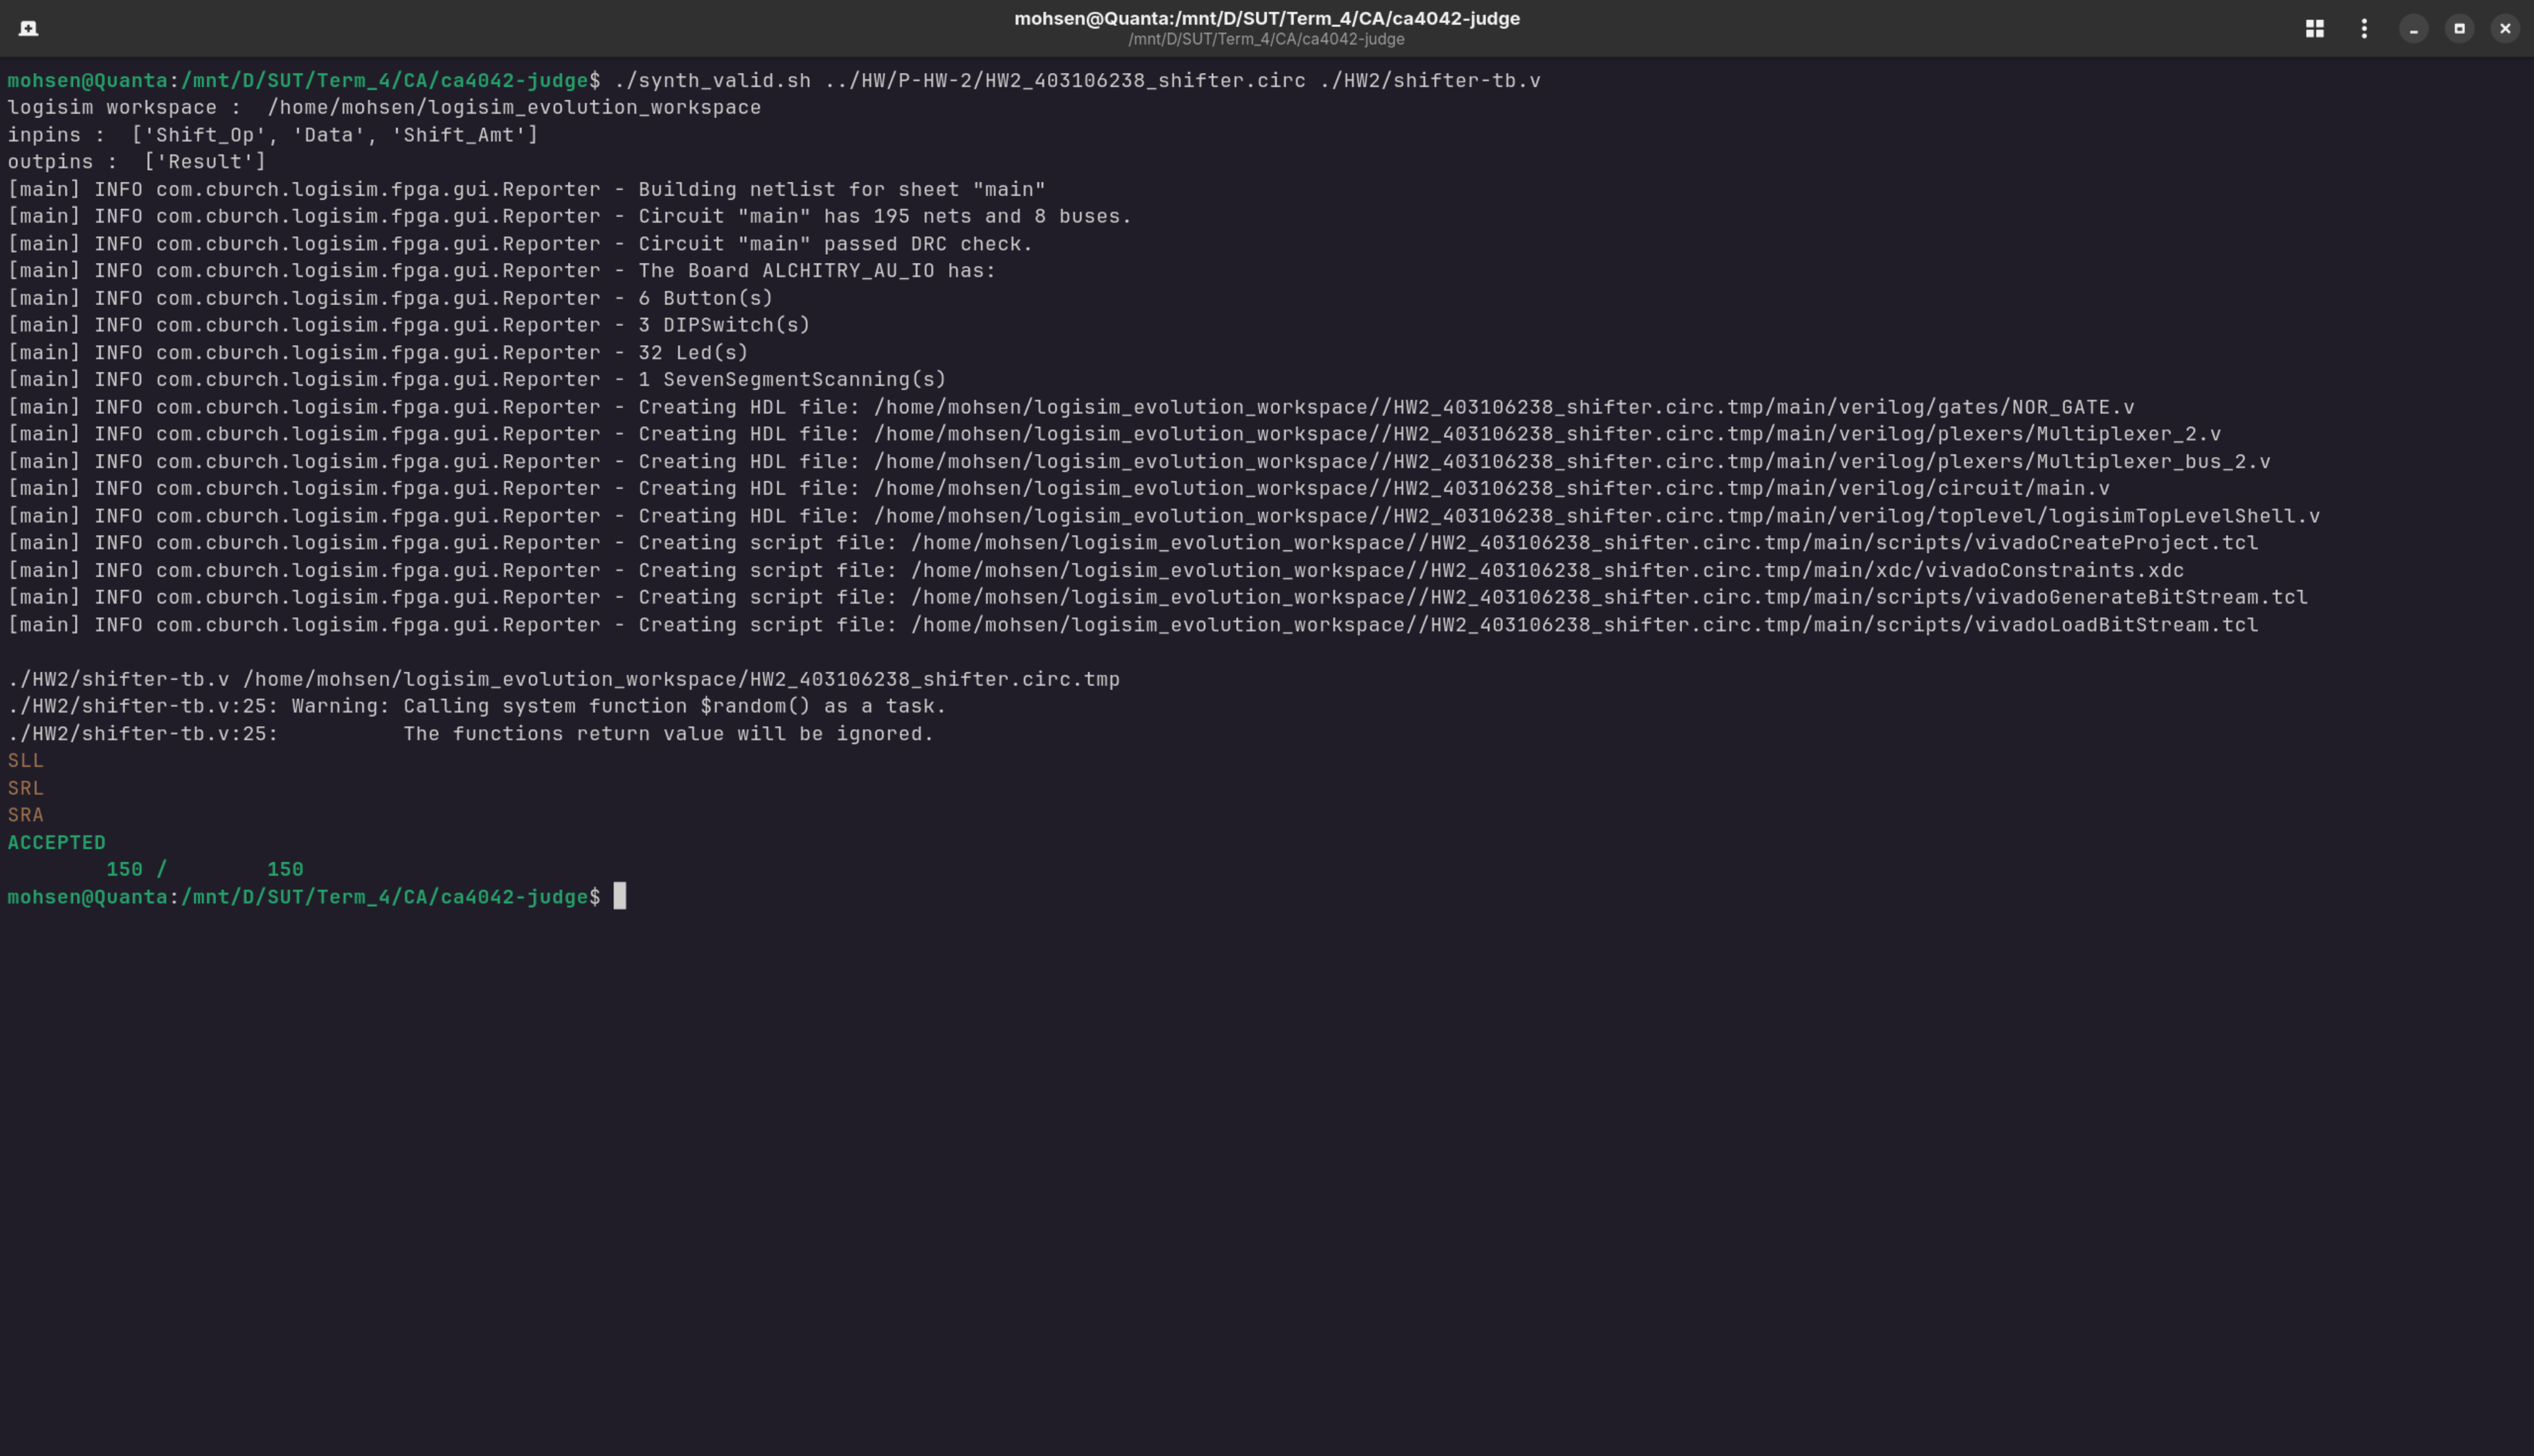
\includegraphics[width=1.0\textwidth]{assets/shifter_test.png}
    \caption{تست مدار طراحی شده}
\end{figure}